\chapter[Resultados Parciais]{Resultados Parciais}

\section{Protótipo inicial}

A fim de atestar a viabilidade do porte do jogo \textit{Traveling Will}, desenvolvido inicialmente para PC, para a plataforma \textit{Nintendo Game Boy Advance}, foi feita uma versão funcional do menu original do jogo, já testada em um \textit{Nintendo DS} (como explicado na seção \ref{console} do capítulo \ref{metodologia}). Para isso, a principal ferramenta utilizada foi a \textit{libtonc}\footnote{\textit{libtonc}, disponível em \url{http://www.coranac.com/files/tonc-code.zip}}, que nessa versão inicial fez o papel de engine do jogo.

Abaixo é possível comparar o menu principal do jogo original com o protótipo implementado sendo executado em um emulador de \textit{Game Boy Advance}:

\begin{figure}[H]
 \centering 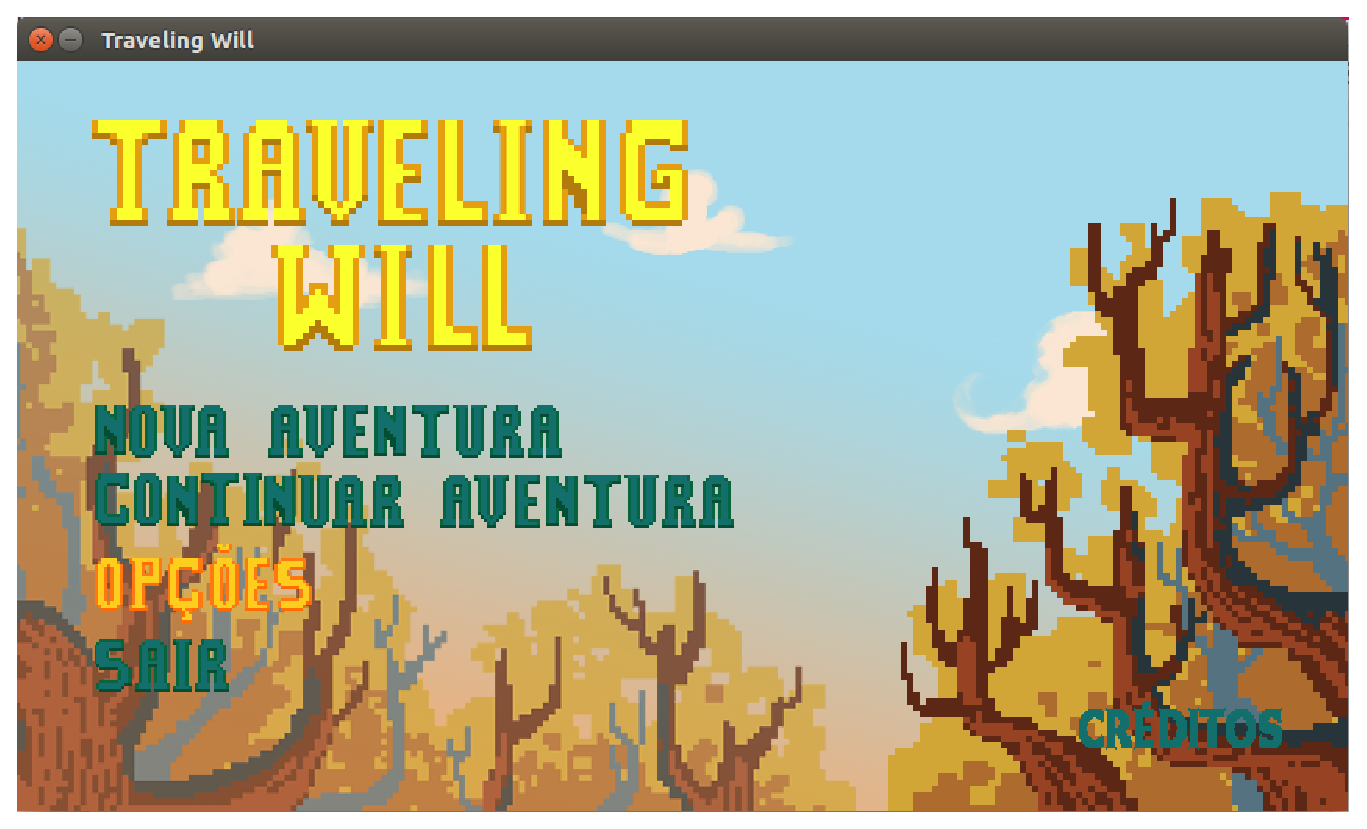
\includegraphics[keepaspectratio=true,scale=0.6]{figuras/tw-original-1.eps}
   \caption[Jogo original sendo executado em um PC]
    {Jogo original sendo executado em um PC. Fonte: \textit{Autores}.}
   \label{tw-original-1}
\end{figure}

\begin{figure}[H]
 \centering 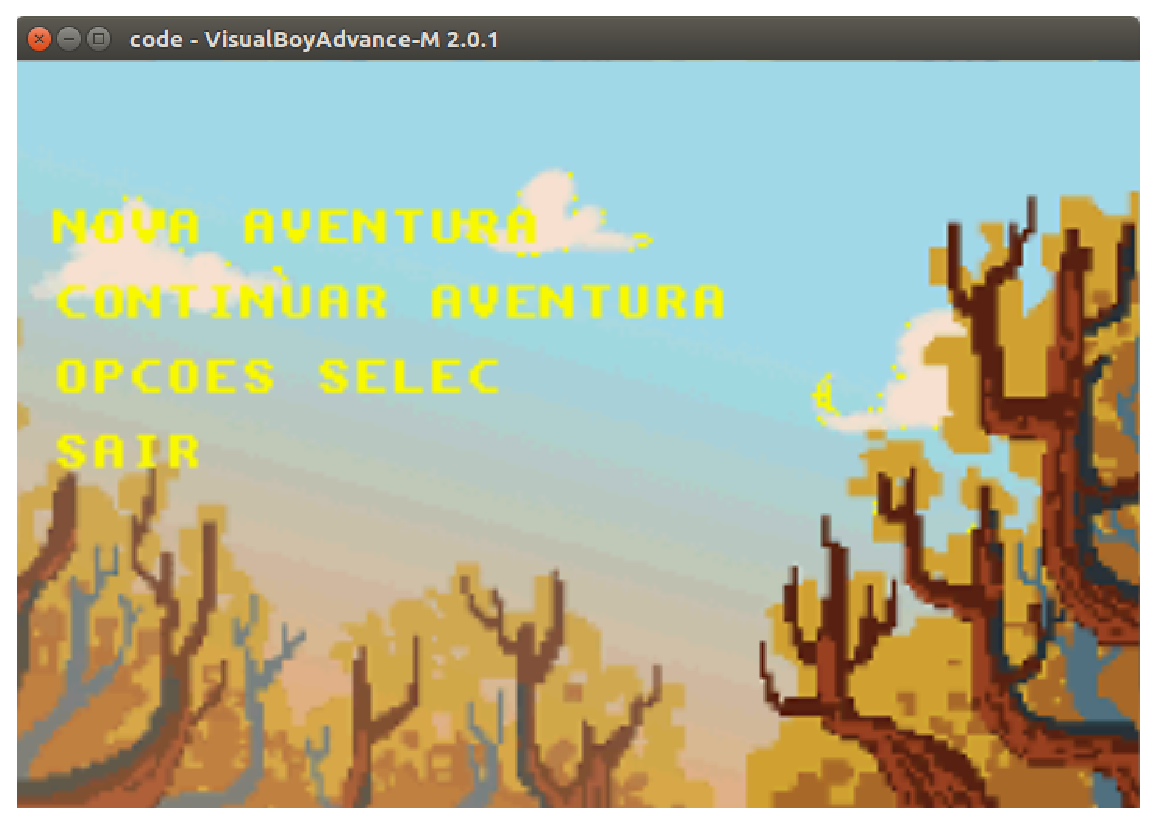
\includegraphics[keepaspectratio=true,scale=0.6]{figuras/tw-gba-1.eps}
   \caption[Protótipo sendo executado no emulador de GBA]
    {Protótipo sendo executado no emulador de GBA. Fonte: \textit{Autores}.}
   \label{tw-gba-1}
\end{figure}

O protótipo desenvolvido está disponível no seguinte repositório: \url{https://github.com/traveling-will-gba/game}

\section{Desenvolvimento da \textit{engine}}

Logo após a finalização do protótipo inicial, foi iniciado o desenvolvimento da \textit{engine} responsável por substituir a \textit{libtonc} e gerenciar os recursos do jogo. Ela foi desenvolvida contendo os seguintes módulos: vídeo, audio, \textit{input} e física. Cada um dos módulos foi desenvolvido tendo como base a \textit{ijengine}... FIXME: Explicar o que é a ijengine.

\subsection{Módulo de \textit{input}}

Os estados dos botões do GBA ficam salvos em um registrador. Cada um desses estados é representado por um \textit{bit} no valor guardado por esse registrador. Sempre que um botão é apertado, o GBA automaticamente troca o valor guardado nesse registrador de tal forma que o \textit{bit} que representa o botão em questão passe a possuir valor 0. De forma similar, quando o botão é solto, o valor contido no \textit{bit} em questão é modificado para 1, seu valor padrão. Sendo assim, a checagem dos estados pode ser realizada facilmente utilizando \textit{bitmasks}. Por exemplo, caso se deseje checar um botão representado pelo \textit{bit} 2 (com a contagem começando em 0), basta pegar o resultado do \textit{AND} binário entre o valor guardado no registrador e a potência de 2 que possui como expotente o \textit{bit} em questão (4, nesse exemplo). Abaixo é possível vizualizar no código do módulo de \textit{input} a definição das constantes que representam os botões, assim como a função utilizada para checar o estado de cada um deles:

\begin{minted}[frame=lines, linenos]
{c++}
#ifndef INPUT\_H
#define INPUT\_H

#include <stdbool.h>
#include "base\_types.h"

#define BUTTON\_A 1
#define BUTTON\_B 2
#define BUTTON\_SELECT 4
#define BUTTON\_START 8
#define BUTTON\_RIGHT 16
#define BUTTON\_LEFT 32
#define BUTTON\_UP 64
#define BUTTON\_DOWN 128
#define BUTTON\_R 256
#define BUTTON\_L 512

#define N\_BUTTON 10

int pressed\_state[N\_BUTTON];

void check\_buttons\_states();
bool pressed(int button);

#endif
\end{minted}
\makebox[\linewidth]{Cabeçalho do módulo de input. Fonte: \textit{Autores}.}
\vspace{\onelineskip}

\begin{minted}[frame=lines, linenos]
{c++}
#include "input.h"

volatile unsigned int *buttons_mem = (volatile unsigned int *)0x04000130;

void check_buttons_states() {
    for(int i = 0; i < N_BUTTON; i++) {
        pressed_state[i] = !((*buttons_mem) & (1 << i));
    }
}

bool pressed(int button) {
    return pressed_state[button];
}
\end{minted}
\makebox[\linewidth]{Código fonte do módulo de input. Fonte: \textit{Autores}.}
\vspace{\onelineskip}

Abaixo é possível visualizar um teste implementado para checar o pressionamento dos botões do GBA. Para cada botão pressionado um \textit{pixel} vermelho aparece na tela. Na imagem abaixo, os botões B, R, \textit{LEFT}, \textit{RIGHT} e \textit{START} estão sendo pressionados simultaneamente.

\begin{figure}[H]
 \centering 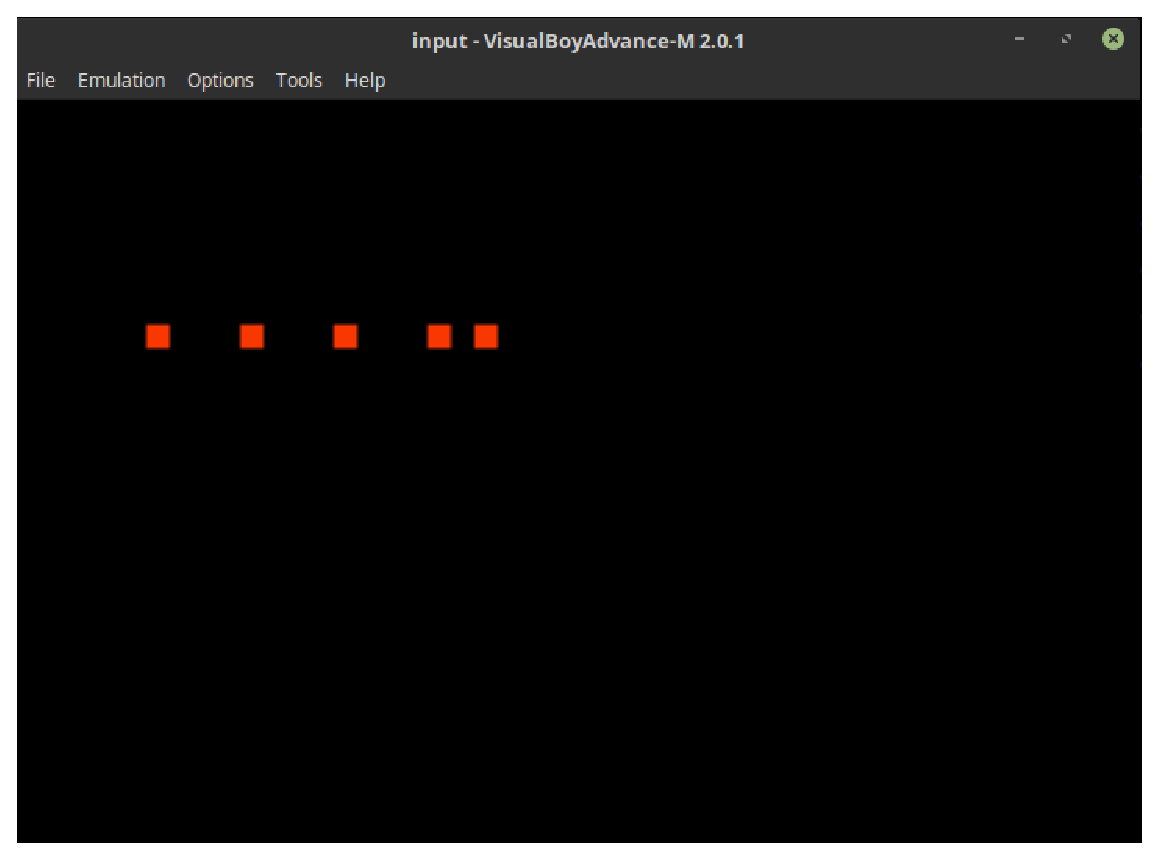
\includegraphics[keepaspectratio=true,scale=0.6]{figuras/demo-input.eps}
   \caption[Demonstração do pressionamento de botões no emulador]
    {Teste de pressionamento de botões no emulador. Fonte: \textit{Autores}.}
   \label{demo-input}
\end{figure}

Abaixo se encontra o código fonte escrito para a realização deste teste:

\begin{minted}[frame=lines, linenos]
{c++}
#include "video.h"
#include "input.h"

#define RED 0x0000FF

unsigned short *vid_mem = (unsigned short *)0x6000000;

int main() {
    reset_dispcnt();
    set_video_mode(3);
    set_background_number(2);

    while(1) {
        check_buttons_states();

        for(int i=0;i<=9;i++){
            if (pressed(i)) {
                vid_mem[50 * 240 + i * 10] = RED;
            } else {
                vid_mem[50 * 240 + i * 10] = 0;
            }
        }
    }

    return 0;
}
\end{minted}
\makebox[\linewidth]{Código fonte do teste de \textit{input}. Fonte: \textit{Autores}.}
\vspace{\onelineskip}

\subsection{Módulo de vídeo}

O módulo de vídeo é responsável pelo controle do modo de vídeo, dos \textit{backgrounds} e da renderização das \textit{sprites}.

Para gerenciar a renderização das \textit{sprites} foi desenvolvida uma classe chamada \textit{Texture}. Ela foi planejada de forma a não apenas copiar os dados da imagem para a região de memória apropriada, mas também permitir a animação das \textit{sprites} de uma textura e controlar os metadados das imagens renderizadas no jogo.

A seguir, será explicado, com o auxílo de trechos do código, o funcionamento dos principais elementos dessa classe.

Inicialmente, é necessário explicar os construtores dessa classe.

Logo abaixo, é possível visualizar o código do primeiro construtor. Ele recebe os ponteiros para a paleta de cores e para o vetor de \textit{tiles} utilizados pela imagem, os tamanhos das regiões de memória alocadas pra cada um desses ponteiros e a quantidade de \textit{bits} por \textit{pixel} que a imagem utiliza. Cada um desses atributos é guardado na própria classe, e, já nesse construtor, são chamados os métodos \textit{set\_sprite\_pal} e \textit{set\_sprite}, responsáveis por copiá-los para as regiões apropriadas. Por fim, ainda nesse construtor, são setados os índices do \textit{tile base} e da paleta de cores utilizada pela imagem. O cálculo desses índices será explicado logo adiante, nos tópicos dedicados aos métodos \textit{set\_sprite\_pal} e \textit{set\_sprite}.

\begin{minted}[frame=lines, linenos]
{c++}
Texture::Texture(uint32_t num_sprites, const uint16_t *pallete, uint32_t pallete_len,
        const unsigned int *tiles, uint32_t tiles_len, enum bits_per_pixel bpp = _8BPP)
{
    this->pallete = pallete;
    this->pallete_len = pallete_len;
    this->pallete_id = 0;
    this->bpp = bpp;
    this->num_sprites = num_sprites;
    this->num_tiles = tiles_len / ((bpp == _4BPP) ? 32 : 64);
    this->tiles_per_sprite = num_tiles / num_sprites;
    this->tiles = tiles;
    this->tiles_len = tiles_len;

    memory_manager = MemoryManager::get_memory_manager();

    set_sprite_pal();
    set_sprite();
    oam_entry = memory_manager->alloc_oam_entry();

    metadata.tid = tile_base * ((bpp == _4BPP) ? 1 : 2);
    metadata.pb = pallete_id;
}
\end{minted}
\makebox[\linewidth]{Código fonte do teste de \textit{input}. Fonte: \textit{Autores}.}
\vspace{\onelineskip}

O segundo construtor funciona de forma similar ao anterior, com a diferença de que em vez de receber todos aqueles atributos da imagem, ele recebe apenas um ponteiro para outra textura. Esse construtor serve para quando se deseja renderizar réplicas de uma mesma textura. Utilizar ele permite que tais texturas compartilhem a paleta de cores e o vetor de \textit{tiles}, fazendo-se necessário alocar espaço apenas para os metadados, que são diferentes pra cada textura.

\begin{minted}[frame=lines, linenos]
{c++}
Texture::Texture(const Texture *texture)
{
    this->num_sprites = texture->num_sprites;
    this->pallete = texture->pallete;
    this->pallete_len = texture->pallete_len;
    this->tiles = texture->tiles;
    this->tiles_len = texture->tiles_len;
    this->bpp = texture->bpp;
    this->pallete_id = texture->pallete_id;
    this->num_tiles = texture->num_tiles;
    this->tiles_per_sprite = texture->tiles_per_sprite;
    this->tile_base = texture->tile_base;

    memory_manager = MemoryManager::get_memory_manager();

    oam_entry = memory_manager->alloc_oam_entry();

    metadata.tid = tile_base * ((bpp == _4BPP) ? 1 : 2);
    metadata.pb = pallete_id;
}
\end{minted}
\makebox[\linewidth]{Código fonte do teste de \textit{input}. Fonte: \textit{Autores}.}
\vspace{\onelineskip}

O método \textit{set\_sprite\_pal} é responsável por chamar o método \textit{alloc\_texture\_pal} da classe \textit{MemoryManager} passando como parâmetro o tamanho da paleta de cores a ser alocada. Como resultado, ele irá receber o endereço de memória aonde a paleta deverá ser guardada. Após fazer a cópia da paleta, é preciso calcular o índice da paleta escolhida na memória, já que esse é um dos metadados necessários para renderização da imagem a 4 \textit{bits} por \textit{pixel}. Como a região reservada para as paletas de cores no \textit{GBA} é divida em regiões de 32 \textit{bytes}, para realizar tal cálculo basta pegar a diferença entre o início da região escolhida para a cópia e o início da região reservada para as paletas e dividir por 32.
Como uma imagem renderizada a 8 \textit{bits} por \textit{pixel} ocupa toda a região reservada para as paletas, o cálculo do índice não é necessário para uma imagem que utilize 256 cores.

\begin{minted}[frame=lines, linenos]
{c++}
bool Texture::set_sprite_pal() {
    volatile uint8_t *teste = memory_manager->alloc_texture_palette(32);
    mem16cpy(teste, pallete, 32);

    this->pallete_id = (teste - (volatile uint8_t *)0x05000200) / 32;

    return true;
}
\end{minted}
\makebox[\linewidth]{Código fonte do teste de \textit{input}. Fonte: \textit{Autores}.}
\vspace{\onelineskip}

O método \textit{set\_sprite} funciona de forma similar ao \textit{set\_sprite\_pal}, tendo como diferença relevante apenas o cálculo do índice do \textit{tile\_base} da imagem, que é feito subtraindo o início da região escolhida para a cópia e o início da região reservada para os \textit{tiles}. Essa diferença ocorre porque diferentemente da paleta de cores, cada unidade do vetor que representa a \textit{tile\_mem} no nosso código é, de fato, um \textit{tile}.

\begin{minted}[frame=lines, linenos]
{c++}
bool Texture::set_sprite() {
    volatile struct tile *teste = memory_manager->alloc_texture(tiles_len);

    mem16cpy((volatile struct tile *)teste, tiles, tiles_len);
    tile_base = teste - memory_manager->base_texture_mem();

    return true;
}
\end{minted}
\makebox[\linewidth]{Código fonte do teste de \textit{input}. Fonte: \textit{Autores}.}
\vspace{\onelineskip}

O método \textit{update\_metadata} apenas copia os metadados para a \textit{OAM} (\textit{Object Attributes Memory}).

\begin{minted}[frame=lines, linenos]
{c++}
void Texture::update_metadata() {
    mem16cpy(oam_entry, &metadata, sizeof(struct attr));
}
\end{minted}
\makebox[\linewidth]{Código fonte do teste de \textit{input}. Fonte: \textit{Autores}.}
\vspace{\onelineskip}

Por fim, o método \textit{update} calcula qual a próxima sprite a ser renderizada e seta o primeiro \textit{tile} dela como \textit{tile\_id}. Esse processo é o que permite a animação das \textit{sprites} do jogo. O cálculo é feito somando o \textit{tile\_id} atual com a quantidade de \textit{tiles} por \textit{sprite} da textura que está sendo renderizada. Vale ressaltar que os índices dos \textit{tiles} são contabilizados sempre de 32 em 32 \textit{bytes}, mesmo que a imagem utilize 8 \textit{bits} por \textit{pixel} e por isso o número de \textit{tiles} por \textit{sprite} é multiplicado por 2 quando o número de \textit{bits} por \textit{pixel} da textura é 8.

Para a renderização dos \textit{backgrounds}, foi desenvolvida uma classe que recebe ponteiros para a paleta de cores,  para o vetor de \textit{tiles} e para o mapa de \textit{tiles} utilizados pelo \textit{background}, assim como os tamanhos das regiões alocadas pra cada um desses ponteiros. Assim que é instanciada, essa classe calcula qual o melhor \textit{charblock} e o melhor \textit{screenblock} para guardar os \textit{tiles} e o mapa de \textit{tiles}, respectivamente. Vale ressaltar que os \textit{charblocks} e \textit{screenblocks} compartilham a mesma região de memória e precisam de um espaço contíguo na memória do \textit{GBA} para que o \textit{background} seja renderizado corretamente. Por esse motivo não é recomendado apenas copiá-los para a memória do \textit{GBA} de forma sequencial, já que isso poderia causar um \textit{overlap} entre um \textit{charblock} e um \textit{screenblock}, e também poderia preencher a memória do \textit{GBA} de forma não-ótima, o que pode fazer com que não caibam todos os \textit{backgrounds} necessários para uma ou mais fases do jogo.

\subsection{Módulo de Física}

O módulo de física é responsável por checar continuamente se os objetos estão colidindo e caso estejam chamar as funções responsáveis por lidar com a colisão para cada objeto. Para realizar tal procedimento esse módulo guarda uma lista de objetos que devem ser considerados na checagem e um ponteiro para o objeto alvo. Dessa forma, sempre que algum objeto colide com o objeto alvo, o método \textit{on\_collision} do alvo e do objeto com o qual ele colidiu é chamado. Logo abaixo, é possível visualizar o código do método responsável por checar se a colisão aconteceu e chamar os métodos \textit{on\_collision} dos objetos envolvidos. 

\begin{minted}[frame=lines, linenos]
{c++}
void Physics::do_collisions() {
    for (auto obj : objects) {
        if (obj == target) continue;

        if (check_collision(target, obj)) {
            target->on_collision(obj);
            obj->on_collision(target);
        }
    }   
}
\end{minted}
\makebox[\linewidth]{Código fonte do teste de \textit{input}. Fonte: \textit{Autores}.}
\vspace{\onelineskip}

Da forma como foi desenvolvido o módulo de física, cada objeto do jogo possui uma \textit{bounding box}, que é uma caixa (retângulo), que representa as extremidades do objeto. Sendo assim, dois objetos estão colidindo somente quando suas caixas possuem uma interseção. Logo abaixo é possível visualizar o método \textit{check\_collision}, responsável por indicar se a colisão entre 2 objetos ocorreu ou não. O método recebe os dois objetos a serem checados, acessa as caixas de cada um e chama o método \textit{intersection}, que é quem de fato vai fazer os cálculos necessários para descobrir se os retângulos possuem ou não uma interseção. Logo abaixo é possível visualizar, respectivamente, os métodos \textit{check\_collision} e o método \textit{intersection}.

\begin{minted}[frame=lines, linenos]
{c++}
bool Physics::check_collision(Collidable *a, Collidable *b) {
    if (not a || not b) return false;
    auto bbA = a->bounding_box();
    auto bbB = b->bounding_box();

    return bbA.intersection(bbB);
}
\end{minted}
\makebox[\linewidth]{Código fonte do teste de \textit{input}. Fonte: \textit{Autores}.}
\vspace{\onelineskip}

\begin{minted}[frame=lines, linenos]
{c++}
bool Rectangle::intersection(const Rectangle& r) const
{
    int xa = x() - w() / 2;
    int xb = x() + w() / 2;
    int xc = r.x() - r.w() / 2;
    int xd = r.x() + r.w() / 2;

    int ya = y() - h() / 2;
    int yb = y() + h() / 2;
    int yc = r.y() - r.h() / 2;
    int yd = r.y() + r.h() / 2;

    pair <int, int> interX = make_pair(max(xa, xc), min(xb, xd));
    pair <int, int> interY = make_pair(max(ya, yc), min(yb, yd));

    return (interX.second - interX.first >=0 && interY.second - interY.first >= -1);
}
\end{minted}
\makebox[\linewidth]{Código fonte do teste de \textit{input}. Fonte: \textit{Autores}.}
\vspace{\onelineskip}

A \textit{engine} desenvolvida está disponível no seguinte repositório: \url{https://github.com/traveling-will-gba/game}
